This is just a chapter running a simulation to see how much money you can make if you quit your full time job and do this for a living.

\section{Running an Arbitrage Betting Operation}

\textbf{Operation:} Use the arbitrage betting method to make money. We start of with an Investment $I$ of R100 per bet we do 10 Arbitrage $A$ bets per day over time $t$. We try and make at least 1\% $ROI$ from each bet. We set our constaints as follows:
$ROI \in [1\% , 3\%]$ \\

Let us see how much money we can make if we do this for a year.\\

We will be putting back the profits in the bets each day so it can be reinvested and profits can grow exponentially.\\

We set up our experiment as follows: \\
    Per bet we use a random function to generate a random number between 1\% and 3\% to determine the ROI of the bet.\\
    We declare a $D_{p}$ variable for profit per day.\\
    We declare a $D_{t}$ variable for total profit over time.\\
    We declare a $D_{i}$ variable for investment per day.\\
    $T$ is set for 365 days.\\

    In reality there is chances of losing money. But for the sake of this experiment we will assume we will always make money.\\
    We could also make more money by doing more bets per day. But for the sake of this experiment we will assume we do 10 bets per day.\\
    The Return on Investment can be always be higher than 3\%. But for the sake of this experiment we will assume $ROI \in [1\% , 3\%]$ \\
    From that we estimate a general formula to create a simulation of the arbitrage betting operation over $T$\\

\begin{equation}
    D_{p} = \begin{cases}
        D_{p} + I \times ROI & \text{if } ROI \in [1\% , 3\%] \\
        D_{p} & \text{if } ROI \notin [1\% , 3\%] \\
    \end{cases}
\end{equation}

Once complete the simulation we can plot the results. Using the simulation we can see how much money we can make if we do this for a year.\\

Once done that we will fit the data into this growth formula here.

\begin{equation}
    D_{t} = I*e^{(D_{p} \times T)}
\end{equation}

 

We can now plot the results of the simulation and the growth formula.

\begin{figure}[H]
    \centering
    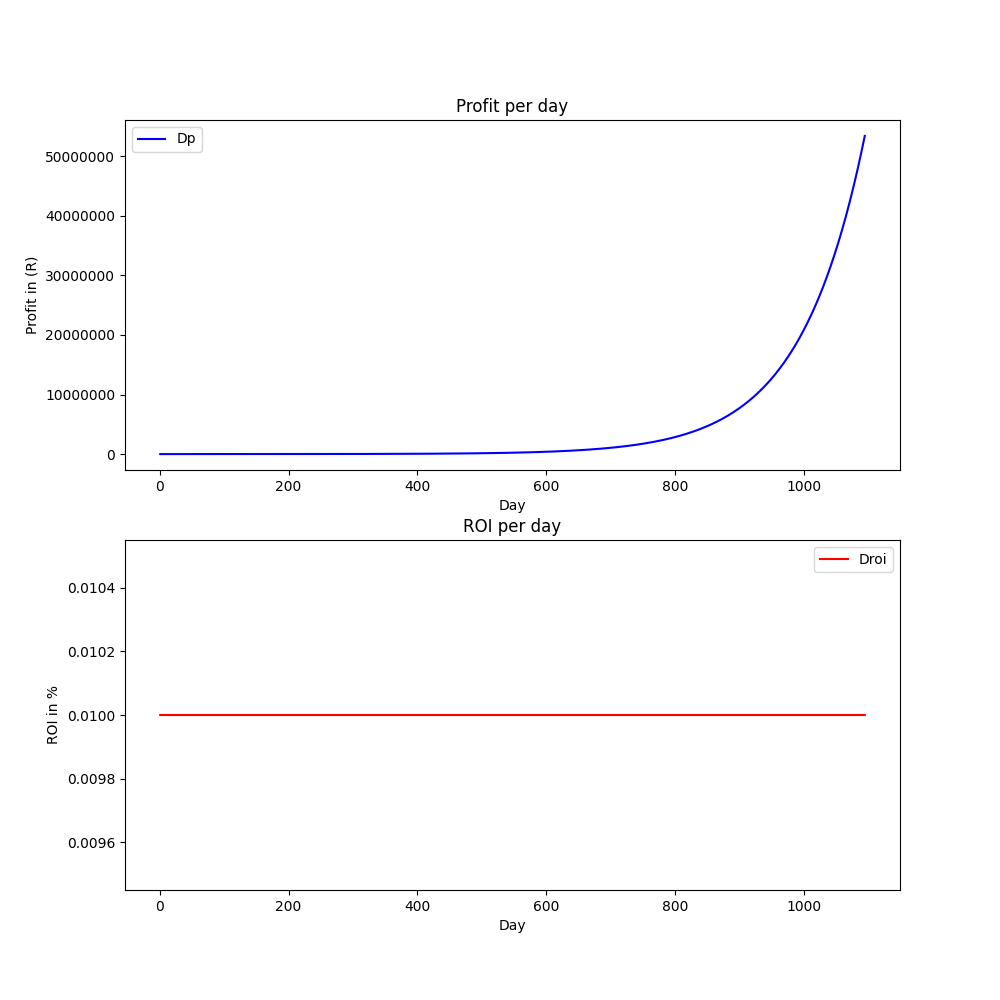
\includegraphics[scale=0.5]{images/plot.png}
    \caption{Plot of the simulation}
    \label{fig:plot}
\end{figure}

\begin{figure}[H]
    \centering
    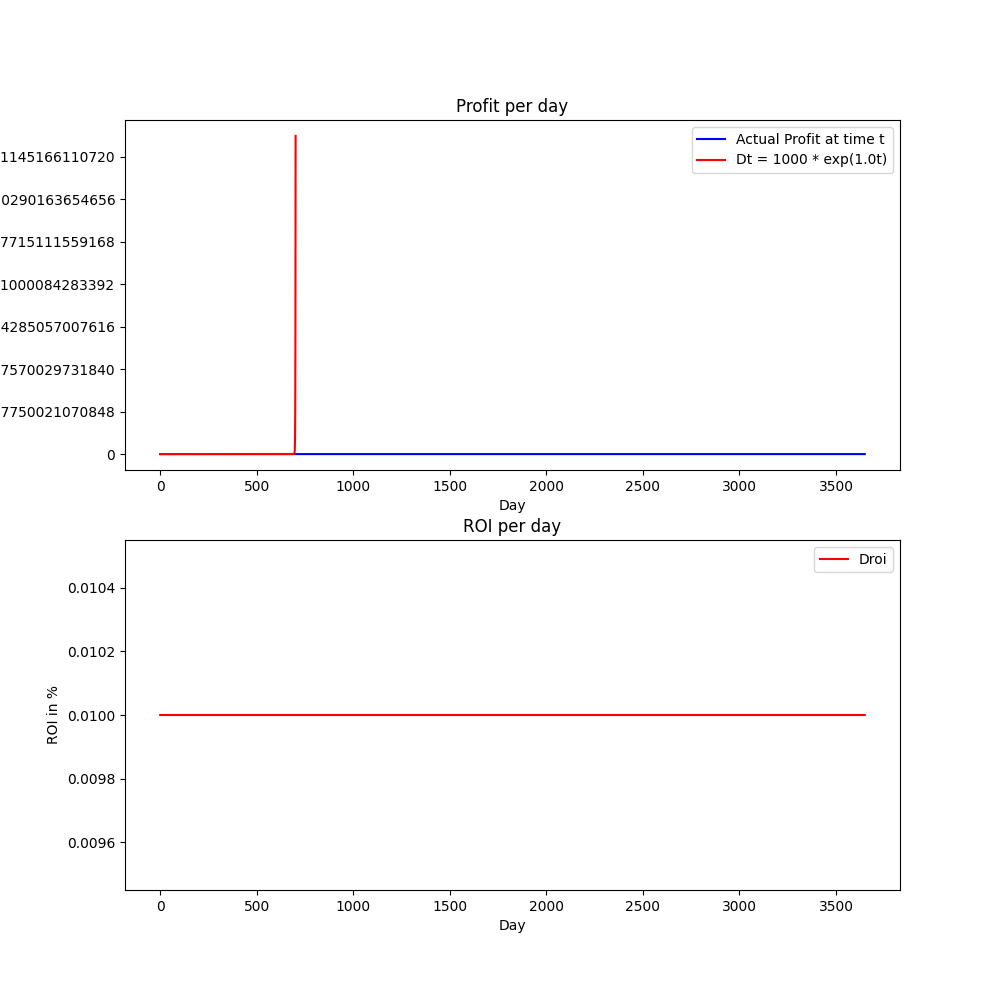
\includegraphics[scale=0.5]{images/fit.png}
    \caption{Plot of the simulation and the growth formula}
    \label{fig:plot2}
\end{figure}

Our best fit is $D_{t} = 1000 \times e^{0.02t}$\\

From this we can see that we can make a lot of money if we do this for a year.\\ 
Starting with an investment R1000 and R100 per bet doing 10 bets a day we can make R1,000,000 in a year.\\

It is also cool to see this model fit the data so well.\\

Running many iterations we can see that our model is very accurate.\\

Therefore we can see that if we increase the investment per bet we can make more money.\\
below is the code for the simulation.

\begin{python}
import random

Dt = 0
I = 1000

Date = []
Dp = []
Droi = []

# get random values from 1%-3% 
def get_random_roi():
    return random.uniform(0.01, 0.03)

for d in range(1, 365):
    Dt = d
    ROI = get_random_roi()
    I = I + (I * ROI)
    Droi.append(ROI)
    Date.append(Dt)
    Dp.append(I)

import seaborn as sns
import matplotlib.pyplot as plt

# plot Date,Dp and Droi sub graphs
fig, (ax1, ax2) = plt.subplots(2, 1, figsize=(10, 10))
ax1.plot(Date, Dp, 'b')
ax1.set_title('Profit per day')
ax1.set_xlabel('Day')
ax1.set_ylabel('Profit in (R)')
ax1.ticklabel_format(useOffset=False, style='plain')
#add legend
ax1.legend(['Dp'])
ax2.plot(Date, Droi, 'r')
ax2.legend(['Droi'])
ax2.set_title('ROI per day')
ax2.set_xlabel('Day')
ax2.set_ylabel('ROI in %')
ax2.ticklabel_format(useOffset=False, style='plain')
#save plot
fig.savefig('images/plot.png')



# curve fit Dp and Droi
import numpy as np
from scipy.optimize import curve_fit

def func(Dp, T):
    return 1000*np.exp(T*Dp)

xdata = np.array(Date)
ydata = np.array(Dp)

popt, pcov = curve_fit(func, xdata, ydata, maxfev=5000)

#print equation
print('Dt = 1000 * exp(T * Dp)')
# print Dt at 1
equation = 'Dt = 1000 * exp('+str(round(popt[0],2))+'t)'

# plot curve fit Dp and Droi sub graphs
fig, (ax1, ax2) = plt.subplots(2, 1, figsize=(10, 10))
ax1.plot(xdata, ydata, 'b', label='data')
ax1.plot(xdata, func(xdata, *popt), 'r-', label='fit')
ax1.set_title('Profit per day')
ax1.set_xlabel('Day')
ax1.set_ylabel('Profit in (R)')
ax1.ticklabel_format(useOffset=False, style='plain')
#add legend
ax1.legend(['Actual Profit at time t', equation])
ax2.plot(Date, Droi, 'r')
ax2.legend(['Droi'])
ax2.set_title('ROI per day')
ax2.set_xlabel('Day')
ax2.set_ylabel('ROI in %')
ax2.ticklabel_format(useOffset=False, style='plain')
plt.show()

#save plot
fig.savefig('images/fit.png')
\end{python}

\section{Conclusion}

In conclusion we can see that we can make a lot of money if we do this for a year. There is also so much risk involved as the odds can change at any time. Multiple bets can also be made at the same time. This can also be done with other sports. If the odds change some losses can be made. But if the odds change in our favour we can make a lot of money.\\ You will have to manage and records where your money is going. This can be done with a spreadsheet or database\\
Finally I will like to tell your that you can get banned from the bookies if you do this. So be careful but there is always ways you can trick the algorithm/system.
I think this could be a good way to make money. But you will have to do a lot of research and testing.\\ This can become a full time job.\\ Once scaled up you can get other people to do the betting for you.\\